\newpage
\newcommand{\mat}[1]{\begin{bmatrix}#1\end{bmatrix}}
\section{Transformations on images}

\subsection{Describing \textbf{TRS} with homogeneous coordinates}

\emph{Please note:} As I understand the task, we are to compute the coordinate
$(x_0\, y_0)$ such that $\tilde{I}(x,\, y) = I(x_0,\ y_0)$.

% To express $\tilde{I}(x,\, y)$ in terms of pixels in $I$, we use
To do so, we first compute
the inverse map $(\mbf{TRS})^{-1}$:


\begin{align*}
  \tilde{I}(x,\, y) &= \ I(x_0,\, y_0)\\[4pt]
  &\text{where } \mat{x_0\\y_0\\1} =
    (\mbf{TRS})^{-1}
    \mat{x\\y\\1}.
\end{align*}
In order to compute $(x_0,\, y_0)$, we first compute the inverse map
$(\mbf{TRS})^{-1}$:
\begin{align*}
  (\mbf{TRS})^{-1} &= 
  \left(
  \mat{1&0&t_x\\0&1&t_y\\0&0&1}
  \mat{\cos \theta&-\sin \theta&0\\\sin \theta&\cos \theta & 0\\0&0&1}
  \mat{s&0&0\\0&s&0\\0&0&1}
  \right)^{-1}\\[8pt]
  &=
  \mat{s \cos \theta & -s \sin \theta & t_x\\
       s \sin \theta & s \cos \theta & t_y\\
       0 & 0 & 1}^{-1}\\[8pt]
  % &=
  % \mat{\frac{\cos t} s  & \frac{\sin t} s & -\frac{t_x \cos \theta + t_y \sin
  % \theta} s\\[12pt]
  % - \frac{\sin \theta} s & \frac{\cos \theta} s & \frac{t_x \sin \theta - t_y
  % \cos \theta} s\\[12pt]
  % 0 & 0 & 1
  % }\\
  &=
  \frac 1 s 
  \mat{\cos \theta   & \sin \theta & -t_x \cos \theta -t_y \sin \theta \\[4pt]
  - \sin \theta & \cos \theta & \quad t_x \sin \theta - t_y \cos \theta\\[4pt]
  0 & 0 & s
  }.
\end{align*}

We then have:
\begin{align*}
  \mat{x_0\\y_0\\1} &= (\mbf{TRS})^{-1}\mat{x\\y\\1}\\
  &=
  \frac 1 s 
  \mat{\cos \theta   & \sin \theta & -t_x \cos \theta -t_y \sin \theta \\[4pt]
  - \sin \theta & \cos \theta &\quad t_x \sin \theta - t_y \cos \theta\\[4pt]
  0 & 0 & s
  } \mat{x\\y\\1}\\
  &=
  \frac 1 s
  \mat{\ \  x \cos \theta + y \sin \theta  - t_x \cos \theta -t_y \sin  \theta\\[4pt]
       -x \sin \theta + y \cos \theta + t_x \sin \theta - t_y \cos \theta\\[4pt]
       s
      }.\\
  % &=
  % \frac 1 s
  % \mat{\cos \theta(x - t_x) + \sin \theta(y + t_y)\\[4pt]
  %      \sin \theta(t_x - x) + \cos \theta(y - t_y)\\[4pt]
  %      s
  %     }.
\end{align*}
Putting it all together, we have:
\begin{align*}
  \tilde{I}(x,\, y)
  &= I\left(
  \frac {\cos \theta(x - t_x)  + \sin \theta (y - t_y)} s ,\
  \frac {\sin \theta (t_x - x) + \cos \theta (y - t_y)} s 
      \right)\\
      &= I(x_0,\, y_0).
\end{align*}
To use nearest neighbor interpolation, we then round $x_0$ and $y_0$ to the
nearest integers:
\begin{align*}
  \tilde{I}(x,\, y) = I\big(\text{round}(x_0),\, \text{round}(y_0)\big).
\end{align*}

\subsection{Transformations in Python}

\Cref{code:my_warp_NN} shows the function I write to perform the transformations
using nearest neighbor interpolation. The function assumes \texttt{f\_inv} is a
$3 \times 3$ inverse map matrix.

\begin{figure}[H]
  \centering
  \begin{minted}[fontsize=\footnotesize]{python}
def my_warp_NN(img, f_inv, cval = 0):

    # array of homogeneous coordinates into img.
    idx1 = np.c_[[*np.ndindex(img.shape)], [1] * img.size].T

    # backward mapped coordinates with NN-interpolation.
    idx2 = (f_inv @ idx1)[:2].T.round().astype(int)

    # mask valid indices.
    mask = ((idx2 >= 0) & (idx2 < img.shape)).all(1)

    # construct result.
    res = np.ones_like(img) * cval
    res[tuple(idx1[:2, mask])] = img[tuple(idx2[mask].T)]
    return res
  \end{minted}
  \captionof{listing}{Image warping using NN-interpolation.}
  \label{code:my_warp_NN}
\end{figure}

Next, \cref{code:transformations} shows the functions I use to construct
transformation matrices $\mbf T$, $\mbf R$, and $\mbf S$, as well as the
combined transformation needed for task 2.2.

\begin{figure}[H]
  \centering
  \begin{minted}[fontsize=\footnotesize]{python}
def T(t):
    return np.c_[np.eye(3, 2), [*t, 1]]

def S(s):
    return np.diag([s, s, 1])

def R(theta):
    cos_t, sin_t = np.cos(theta), np.sin(theta)
    return np.array([[cos_t, -sin_t, 0], [sin_t, cos_t, 0], [0, 0, 1]])

def task_2_2_transformation(center, t, theta, s):
    Tc = T(center)
    return T(t) @ Tc @ R(theta) @ S(s) @ np.linalg.inv(Tc)
  \end{minted}
  \captionof{listing}{Transformation matrices.}
  \label{code:transformations}
\end{figure}

Finally, \cref{code:task_2_2} shows the code used to generate the example
described in the assignment text, while \cref{fig:task_2_2} shows the actual
result.
\begin{figure}[H]
  \centering
  \begin{minted}[fontsize=\footnotesize]{python}
img = np.zeros((100, 100))
img[40:60, 40:60] = 1

center = np.asarray(img.shape) // 2
t, theta, s = (10.4, 15.7), np.pi / 10, 2

f   = task_2_2_transformation(center, t, theta, s)
res = my_warp_NN(img, np.linalg.inv(f))
  \end{minted}
  \captionof{listing}{Code for generating \cref{fig:task_2_2}.}
  \label{code:task_2_2}
\end{figure}

\begin{figure}[H]
  \centering
  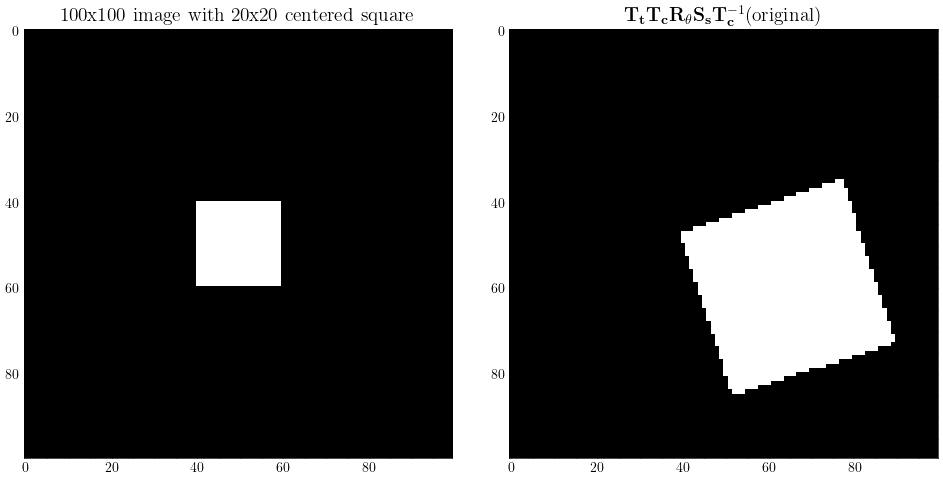
\includegraphics[width=\textwidth]{figures/task_2_2.png}
  \caption{100x100 black image with centered 20x20 white pixels, and the same
  image warped using $\mbf{T_tT_cR}_\theta\mbf{S_sT_c}^{-1}$.}
  \label{fig:task_2_2}
\end{figure}
